\documentclass{standalone}
\usepackage{tikz}

\begin{document}

\centering

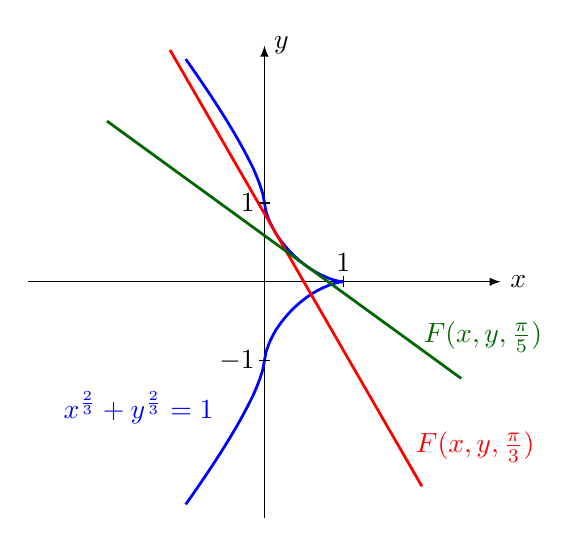
\begin{tikzpicture}
    % draw axes
    \coordinate (O) at (0,0);
    \draw[-latex] (0,-3) -- (0,3) node[anchor=west] {$y$};
    \draw[-latex] (-3,0) -- (3,0) node[anchor=west] {$x$};

    % draw curves
    \def\a{1} % constant

    \draw[blue,domain=-1:1,samples=50, line width=1] plot ({\x},{(1-\x^(2/3))^(3/2)});

    \node[blue,align=left] at (-1.6,-1.6) {$x^{\frac{2}{3}} + y^{\frac{2}{3}} = 1$};

    \draw[blue,domain=-1:1,samples=50, line width=1] plot ({\x},{-(1-\x^(2/3))^(3/2)});
    
    \draw[red,domain=-1.2:2, samples=100, line width=1] plot ({\x}, {(1-\x/cos(pi/3 r))*sin(pi/3 r)});
    \node[anchor=west] at (1.8,-2.1) {\textcolor{red}{$F(x,y, \frac{\pi}{3})$}};

    \draw[black!60!green,domain=-2:2.5, samples=100, line width=1] plot ({\x}, {(1-\x/cos(pi/5 r))*sin(pi/5 r)});
    \node[anchor=west] at (1.9,-0.7) {\textcolor{black!60!green}{$F(x,y, \frac{\pi}{5})$}};

    % draw labels
    \node[anchor=east] at (0,-1) {$-1$};
    \draw (-2pt,-1) -- (2pt,-1);
    
    \node[anchor=east] at (0,1) {$1$};
    \draw (-2pt,1) -- (2pt,1);

    \node[anchor=south] at (1,0) {$1$};
    \draw (1,-2pt) -- (1,2pt);
    
\end{tikzpicture}
\end{document}